% ============================================================================
%  SECTION 3 — LECTURE NOTES
%  The Philosophy of Machine Minds
%  Comprehensive instructor notes for presentation delivery
% ============================================================================
\documentclass[11pt, a4paper]{article}

\usepackage[margin=2.5cm]{geometry}
\usepackage{amsmath, amssymb, amsthm}
\usepackage{tikz}
\usetikzlibrary{arrows.meta, positioning, calc}
\usepackage{booktabs}
\usepackage{enumitem}
\usepackage{hyperref}
\usepackage[dvipsnames]{xcolor}
\usepackage{tcolorbox}
\usepackage{microtype}
\usepackage{parskip}
\usepackage{titlesec}
\usepackage{fancyhdr}
\usepackage{marginnote}

% --- Colours ---
\definecolor{accent}{HTML}{BF360C}
\definecolor{muted}{HTML}{546E7A}
\definecolor{boxbg}{HTML}{FFF3E0}
\definecolor{defbg}{HTML}{E3F2FD}
\definecolor{warnbg}{HTML}{FCE4EC}

% --- Boxes ---
\tcbuselibrary{breakable, skins}

\newtcolorbox{keyinsight}[1][]{%
  colback=boxbg, colframe=accent, fonttitle=\bfseries,
  title={Key Insight}, breakable, #1}

\newtcolorbox{definition}[1][]{%
  colback=defbg, colframe=MidnightBlue, fonttitle=\bfseries,
  title={Definition}, breakable, #1}

\newtcolorbox{speakingnote}[1][]{%
  colback=gray!8, colframe=muted, fonttitle=\bfseries\color{muted},
  title={Speaking Note}, breakable, left=4mm, right=4mm, #1}

\newtcolorbox{warning}[1][]{%
  colback=warnbg, colframe=Red, fonttitle=\bfseries,
  title={Caution}, breakable, #1}

% --- Headers ---
\pagestyle{fancy}
\fancyhf{}
\fancyhead[L]{\small\textsc{Section 3 --- The Philosophy of Machine Minds}}
\fancyhead[R]{\small\thepage}
\renewcommand{\headrulewidth}{0.4pt}

% --- Title formatting ---
\titleformat{\section}{\Large\bfseries\color{accent}}{}{0em}{}[\vspace{-0.3em}\rule{\textwidth}{0.8pt}]
\titleformat{\subsection}{\large\bfseries}{}{0em}{}

% --- Meta ---
\title{\textbf{Lecture Notes}\\[0.3em]
  \LARGE The Philosophy of Machine Minds\\[0.2em]
  \large Prediction, Representation, and Understanding\\
  in the Age of Large Language Models}
\author{Section 3 --- Executive AI Programme}
\date{2026}

% ============================================================================
\begin{document}
\maketitle
\thispagestyle{empty}

\vspace{1em}
\begin{center}
\begin{tcolorbox}[colback=gray!5, colframe=black, width=0.85\textwidth]
\textbf{Session duration:} 30 minutes (25 min presentation + 5 min discussion)\\
\textbf{Narrative arc:} Mathematical identity $\to$ cosmic empirical observation $\to$ oldest open question in philosophy of mind\\
\textbf{Unifying thread:} \emph{LLMs are forcing us to redefine what it means to understand.}
\end{tcolorbox}
\end{center}

\tableofcontents
\newpage

% ============================================================================
\section{Opening: The Arc of the Argument}
% ============================================================================

This session is structured as a single argument in three acts. Each act
builds on the previous one, and the conclusion of the third act depends on
having internalised the first two.

\textbf{Act I} (Topic A) establishes a mathematical identity: prediction,
compression, and intelligence are the same operation, viewed from different
angles. This is not metaphor --- it is a theorem-level claim traceable to
Shannon (1948), Kolmogorov (1963), Solomonoff (1964), and Hutter (2005).

\textbf{Act II} (Topic B) presents an empirical observation that follows
naturally from Act I: if all powerful learning systems are compressing
reality, they should converge on similar internal representations. The
Platonic Representation Hypothesis (Huh et al., ICML 2024) provides
evidence that this is exactly what is happening.

\textbf{Act III} (Topic C) confronts the philosophical consequence: if
models compress, build world models, and converge on reality's structure,
can we still deny that they ``understand''? The Chinese Room argument
(Searle, 1980) says yes. Recent empirical evidence says: it's complicated.

\begin{speakingnote}
Open with energy and promise. The audience should feel that this session
will change how they think about a fundamental concept. Say something like:
``This session is different from what came before. We've seen what LLMs can
do. Now we confront what those capabilities \emph{mean}. By the end, you
may find that the word `understanding' --- a word you use fifty times a
day --- no longer means what you thought it did.''
\end{speakingnote}

% ============================================================================
\section{Topic A: Prediction = Compression = Intelligence}
% ============================================================================

\subsection{Opening Hook: The Fibonacci Compression}

Display the sequence: $1, 1, 2, 3, 5, 8, 13, \;?$

Pause. Let the audience's brains do the work. Then:

\begin{quote}
``You just replaced an infinite list with a two-word rule: \emph{add the
previous two}. That act of compression \textbf{is} understanding. Your
brain is, at its core, a compression engine.''
\end{quote}

This is the intuitive version of the entire Topic A argument. The rest of
this section makes it rigorous.

\begin{speakingnote}
Do not rush past this moment. The Fibonacci example is doing real
intellectual work --- it is establishing the intuition that compression and
understanding are not merely related, but identical. Everything that follows
is a formalisation of what the audience just experienced in their own heads.
\end{speakingnote}


\subsection{Shannon's Foundational Result (1948)}

\begin{definition}[title={Shannon Entropy}]
For a discrete random variable $X$ with probability mass function $p$,
the \textbf{Shannon entropy} is:
\[
H(X) = -\sum_{x} p(x) \log_2 p(x)
\]
This is the theoretical minimum number of bits required, on average, to
encode one sample from $X$. It is simultaneously a measure of uncertainty
(how surprised you will be) and compressibility (how short your codes can be).
\end{definition}

Shannon's 1948 paper, ``A Mathematical Theory of Communication,'' proved
that the optimal code length for a symbol $x_t$ given its history $x_{<t}$
is:
\[
\ell^*(x_t) = -\log_2 p(x_t \mid x_{<t})
\]

This equation is the linchpin of the entire argument. Unpack it carefully
for the audience:

\begin{itemize}[leftmargin=2em]
  \item If you can \textbf{predict} the next symbol with high probability
    (i.e., $p(x_t \mid x_{<t})$ is close to 1), then $-\log_2 p$ is
    small, so the optimal code is \textbf{short}. You have compressed the
    data.

  \item If you \textbf{cannot} predict the next symbol (i.e., the
    distribution is close to uniform), then $-\log_2 p$ is large, and
    you need many bits. You cannot compress.

  \item Therefore: \textbf{better prediction $\Leftrightarrow$ better
    compression.} These are not two related tasks --- they are the
    \emph{same} mathematical operation expressed in dual form.
\end{itemize}

\begin{keyinsight}
Shannon's result means that any system that does next-token prediction is
\emph{implicitly} performing data compression. When we train an LLM to
minimise cross-entropy loss, we are literally training it to be a better
compressor. The training objective $\mathcal{L} = -\frac{1}{T}\sum_{t=1}^T
\log p_\theta(x_t \mid x_{<t})$ is the average code length under the
model's distribution. Minimising this loss means minimising the number of
bits needed to encode the training data.
\end{keyinsight}

\subsection{The Theoretical Chain: Solomonoff, Kolmogorov, Hutter}

Shannon established prediction $=$ compression. The next link in the chain
connects compression to intelligence itself. This requires three theorists:

\textbf{Kolmogorov Complexity} (Kolmogorov, 1963; Solomonoff, 1960; Chaitin, 1966):

\begin{definition}[title={Kolmogorov Complexity}]
The \textbf{Kolmogorov complexity} $K(x)$ of a string $x$ is the length
of the shortest program (on a fixed universal Turing machine) that outputs
$x$ and halts:
\[
K(x) = \min_{p:\; U(p) = x} |p|
\]
This is the ultimate compression: find the shortest possible description
of the data.
\end{definition}

Kolmogorov complexity is uncomputable (this is a theorem, related to the
halting problem). But it provides the theoretical ideal that all
compression algorithms approximate.

\textbf{Solomonoff Induction} (Solomonoff, 1964):

Solomonoff showed that the optimal way to predict the next symbol in a
sequence is to consider \emph{all} possible programs that could generate
the observed prefix, weighted by their length (shorter programs get
exponentially more weight). This is a Bayesian mixture over computable
hypotheses:
\[
p_{\text{Sol}}(x_{t+1} \mid x_{\leq t}) = \sum_{\text{programs } q:\;
q \text{ outputs } x_{\leq t}\ldots} 2^{-|q|}
\cdot \mathbb{1}[q \text{ outputs } x_{t+1} \text{ next}]
\]
(Simplified; the actual formulation uses a universal semimeasure.)

Solomonoff induction is the theoretically optimal predictor. It is also
uncomputable. But it establishes the \emph{identity}: optimal prediction
= optimal compression = Bayesian reasoning over all possible explanations.

\textbf{AIXI} (Hutter, 2000, 2005):

Marcus Hutter extended Solomonoff induction to the \emph{agent} setting.
AIXI is a theoretical agent that:
\begin{enumerate}[leftmargin=2em]
  \item Maintains a Solomonoff-style model of the environment
  \item Selects actions that maximise expected future reward
  \item Achieves theoretically optimal performance in \emph{any}
    computable environment
\end{enumerate}

\begin{keyinsight}
The AIXI result closes the chain:

\begin{center}
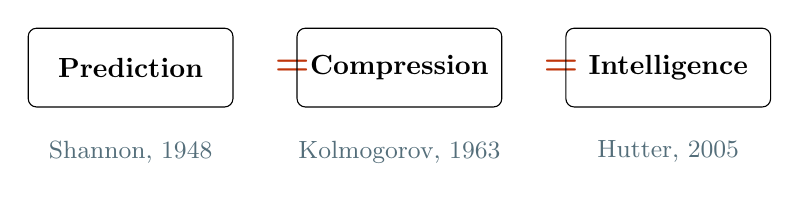
\begin{tikzpicture}[
    box/.style={draw, rounded corners=3pt, minimum width=2.6cm,
                minimum height=1cm, align=center, font=\bfseries},
    eq/.style={font=\Large\bfseries, text=accent}
  ]
  \node[box] (pred) {Prediction};
  \node[eq, right=0.4cm of pred] {=};
  \node[box, right=0.8cm of pred] (comp) {Compression};
  \node[eq, right=0.4cm of comp] {=};
  \node[box, right=0.8cm of comp] (intel) {Intelligence};

  \node[below=0.3cm of pred, font=\small, text=muted] {Shannon, 1948};
  \node[below=0.3cm of comp, font=\small, text=muted] {Kolmogorov, 1963};
  \node[below=0.3cm of intel, font=\small, text=muted] {Hutter, 2005};
\end{tikzpicture}
\end{center}

The perfect compressor is the most intelligent possible agent. Not by
analogy, but by mathematical proof. This means that every improvement in
next-token prediction is an improvement in \emph{general intelligence},
in the precise Hutter sense.
\end{keyinsight}

\begin{speakingnote}
For this audience, you do not need to derive Solomonoff induction.
The key message is: ``There is a chain of mathematical results, published
over 60 years, that proves prediction, compression, and intelligence are
the same thing. This is not a metaphor. It is as rigorous as the claim that
addition and subtraction are inverse operations.''
\end{speakingnote}


\subsection{The Empirical Bombshell: Language Modeling Is Compression}

D\'{e}letang et al.\ (ICLR 2024, Google DeepMind, arXiv:2309.10668)
performed a deceptively simple experiment: they used language models as
general-purpose compressors and compared them to domain-specific
compression algorithms.

\textbf{Method.} Any probabilistic model $p_\theta$ can be turned into a
compressor via arithmetic coding: encode symbol $x_t$ using
$-\log_2 p_\theta(x_t \mid x_{<t})$ bits. The better the model predicts,
the fewer bits it uses. D\'{e}letang et al.\ fed raw bytes of images
(ImageNet patches) and audio (LibriSpeech) through Chinchilla 70B --- a
model trained \emph{exclusively on text} --- and measured the resulting
compression ratios.

\textbf{Results:}

\begin{center}
\begin{tabular}{lcc}
\toprule
\textbf{Domain} & \textbf{Specialist Compressor} & \textbf{Chinchilla 70B} \\
\midrule
Images (ImageNet)  & PNG: 58.5\% & \textbf{43.4\%} \\
Audio (LibriSpeech) & FLAC: 30.3\% & \textbf{16.4\%} \\
\bottomrule
\end{tabular}
\end{center}
\small{(Compression ratio = compressed size / original size. Lower is better.)}
\normalsize

\begin{keyinsight}
Chinchilla 70B has never seen a photograph. It has never heard a sound.
It was trained on text and text alone. Yet it compresses images better
than PNG (an algorithm \emph{designed} for images) and audio better than
FLAC (an algorithm \emph{designed} for audio).

This is not a parlour trick. It means that next-token prediction on text
forced the model to learn something \emph{universal} about the statistical
structure of data --- structure that transfers across modalities the model
was never exposed to.
\end{keyinsight}

\textbf{Why does this work?} The intuition is that all structured data ---
images, audio, text, code --- shares deep statistical regularities.
Natural images have spatial correlations (nearby pixels are similar),
frequency structure (smooth regions with sharp edges), and semantic
structure (objects, textures). Audio has temporal correlations, harmonic
structure, and phonemic patterns. Text describes all of these things. A
model that deeply understands the \emph{structure of descriptions} of
images has, in some sense, learned the structure of images themselves.

More formally: if the model learns a good approximation to the universal
prior (the Solomonoff distribution), it should compress \emph{any}
computable data well, regardless of domain. The D\'{e}letang result
suggests that large language models are, in fact, approximating something
close to a universal compressor.

\textbf{Connection to scaling laws.} Kaplan et al.\ (2020) showed that
language model loss (= compression rate) follows clean power laws in
model size, dataset size, and compute:
\[
L(N) \approx \left(\frac{N_c}{N}\right)^{\alpha_N}
\]
where $N$ is the number of parameters and $\alpha_N \approx 0.076$.
These power laws \emph{are} compression improvement curves. Each order of
magnitude in scale buys a predictable, diminishing improvement in
compression. The scaling laws tell us that we are on a smooth trajectory
toward better and better approximations of the universal compressor.


\subsection{The Philosophical Punchline of Topic A}

\begin{quote}
\emph{If compression is understanding, and LLMs are the best compressors
we have ever built, then the ``stochastic parrot'' critique is not just
wrong --- it is incoherent.}
\end{quote}

This is a strong claim. Unpack it:

The ``stochastic parrot'' framing (Bender et al., 2021) argues that LLMs
are merely doing sophisticated pattern matching without genuine
understanding. But if the Shannon--Hutter chain is correct, then
``pattern matching'' at the level of a universal compressor \textbf{is}
the most general form of intelligence. There is no ``genuine
understanding'' that is separate from, or above, perfect compression.

\begin{warning}
This conclusion is logically valid \emph{given} the premises. But the
premises are debatable:
\begin{enumerate}[leftmargin=2em]
  \item Hutter's framework defines intelligence in terms of
    compression/prediction. Other definitions exist (embodied cognition,
    phenomenal consciousness, social intelligence).
  \item LLMs are finite approximations to the Solomonoff ideal. The gap
    between the approximation and the ideal may be where ``real''
    understanding lives.
  \item Compression is necessary for intelligence, but it may not be
    \emph{sufficient}. A perfect compressor might still lack something ---
    intentionality, consciousness, grounding.
\end{enumerate}
Do \textbf{not} present the compression = understanding claim as settled
fact. Present it as a serious theoretical argument with strong empirical
support that demands engagement. The audience should leave \emph{unsettled},
not convinced.
\end{warning}

\begin{speakingnote}
The right tone for the transition is: ``I have shown you a mathematical
identity and a shocking empirical result. The implication seems to be that
LLMs genuinely understand. But I want you to hold that conclusion lightly,
because I am about to show you something that makes it even stranger ---
and then something that complicates it.''
\end{speakingnote}


% ============================================================================
\section{Topic B: The Platonic Representation Hypothesis}
% ============================================================================

\subsection{Opening: Plato's Allegory of the Cave}

Before presenting any empirical results, set the philosophical frame.

Plato's \emph{Republic}, Book VII (c.\ 375 BCE): Prisoners chained in a
cave see only shadows on the wall. They take the shadows for reality. One
prisoner escapes, sees the sun and real objects, and realises the shadows
were mere projections of a deeper reality.

Plato's metaphysics posits a ``realm of Forms'' --- perfect, abstract
templates of which physical objects are imperfect copies. A chair is a
chair because it participates in the Form of Chair-ness. This view has
been debated for 2,400 years.

\begin{speakingnote}
``Plato argued 2,400 years ago that behind the messy world of appearances
lies a realm of perfect Forms. Philosophers have been arguing about it
ever since. In 2024, a team at MIT published evidence that AI models are
converging on the same internal representation of reality --- regardless
of who built them, what data they trained on, or what architecture they
used. Plato, it turns out, may have been writing about neural networks.''
\end{speakingnote}


\subsection{The Hypothesis (Huh et al., ICML 2024)}

Huh, Cheung, Wang, and Isola (MIT) published ``The Platonic Representation
Hypothesis'' as a position paper at ICML 2024 (arXiv:2405.07987). Their
central claim:

\begin{keyinsight}[title={The Platonic Representation Hypothesis}]
As AI models increase in scale and capability, their learned
representations converge toward a shared statistical model of reality,
regardless of:
\begin{itemize}[leftmargin=2em]
  \item The training data (text, images, audio, video, code)
  \item The architecture (Transformer, CNN, diffusion model, etc.)
  \item The training objective (next-token prediction, contrastive
    learning, masked image modelling, etc.)
  \item The organisation that built the model
\end{itemize}
The hypothesis is that there exists a unique ``correct'' representation
of reality's statistical structure, and all sufficiently powerful learners
discover it.
\end{keyinsight}

\textbf{Evidence presented by Huh et al.:}

\begin{enumerate}[leftmargin=2em]
  \item \textbf{Cross-model alignment increases with scale.} When you
    measure the similarity of internal representations between pairs of
    models (using metrics like CKA --- Centred Kernel Alignment, or
    mutual nearest neighbours), the similarity \emph{increases} as both
    models get larger. Small models are idiosyncratic; large models
    converge.

  \item \textbf{Cross-modality alignment.} Vision models and language
    models, despite processing entirely different data types, develop
    increasingly aligned representation spaces. A concept like ``dog''
    occupies a similar geometric position in the representation space of
    a vision model and a language model.

  \item \textbf{The ``kernel hypothesis.''} Huh et al.\ argue that the
    convergence point is the statistical structure of reality itself ---
    specifically, the kernel of the joint distribution over all possible
    sensory modalities. If you had access to the full joint distribution
    $p(\text{text}, \text{image}, \text{audio}, \text{video},$ $\ldots)$,
    its structure would determine a unique (up to isomorphism)
    representation. All models are approximating this structure from
    different marginals.
\end{enumerate}


\subsection{Evidence: Othello-GPT and Emergent World Models}

Li et al., ``Emergent World Representations: Exploring a Sequence Model
Trained on a Synthetic Task'' (ICLR 2023).

\textbf{Setup:} A GPT-style Transformer is trained on sequences of legal
Othello moves, represented as coordinate pairs (e.g., ``d3 c5 f6\ldots'').
The model receives:
\begin{itemize}[leftmargin=2em]
  \item No description of the Othello board
  \item No encoding of the rules
  \item No visual representation of game states
  \item Only raw move sequences
\end{itemize}

\textbf{Finding:} Using non-linear probes on the model's internal
activations, Li et al.\ found that the model develops a representation
of the full $8 \times 8$ board state --- which cells are black, white,
or empty --- that is accurate at each point in the game.

\textbf{The Nanda refinement (2023):} Neel Nanda showed that the board
representation is not merely present in a tangled, non-linear form. It
is \emph{linearly} decodable: a simple linear probe (a matrix
multiplication) can extract the board state from the model's activations
with high accuracy. This is significant because linear representations
are interpretable, robust, and suggest genuine structural understanding
rather than a memorised lookup table.

\begin{keyinsight}
The model \emph{inferred the existence of a world it was never shown}.
It was trained to predict the next move in a sequence. From that
prediction task alone, it constructed an internal model of the hidden
state that generates the sequence. This is exactly what the
prediction--compression--intelligence chain predicts: to compress move
sequences optimally, you need to discover the latent structure (the
board) that generates them.
\end{keyinsight}

\begin{speakingnote}
Emphasise the wonder here: ``A model trained on sequences of Othello
moves --- just coordinate pairs --- was never told that a board exists,
or what the rules are. Inside its weights, researchers found a clean,
linear representation of the board state. The model inferred the existence
of a world it was never shown. If that doesn't make you pause, I don't
know what will.''
\end{speakingnote}


\subsection{Evidence: Space and Time Neurons}

Gurnee and Tegmark, ``Language Models Represent Space and Time'' (ICLR 2024).

\textbf{Setup:} The authors probed the internal activations of Llama-2
(a large language model trained on text) when it processed sentences
containing geographic locations (cities, countries) and historical dates.

\textbf{Findings:}

\begin{enumerate}[leftmargin=2em]
  \item \textbf{Space neurons:} Individual neurons in Llama-2 activate
    in proportion to the latitude or longitude of the location mentioned
    in the input text. There are neurons whose activation is a linear
    function of geographic coordinates. The model has built an internal
    coordinate system --- essentially, a map --- from text alone.

  \item \textbf{Time neurons:} Similarly, individual neurons encode
    historical dates on a linear timeline. The activation is proportional
    to the year associated with the entity or event in the text.

  \item \textbf{Linearity:} Both spatial and temporal representations are
    \emph{linear} --- they can be extracted by simple linear probes. This
    mirrors the Othello-GPT finding and suggests a general principle:
    language models build clean, structured, linear models of latent
    variables that govern their training data.
\end{enumerate}

\textbf{Interpretation:} The model was never shown a map, a globe, or a
timeline. It learned spatial and temporal structure purely from the
statistical regularities of text --- which cities are mentioned together,
which events co-occur, how descriptions of weather, culture, and
geography cluster. The model discovered that the latent generating
structure behind these textual patterns is a spatial coordinate system
and a temporal axis.

This connects directly to the Platonic Representation Hypothesis: the
model is recovering the \emph{actual structure of reality} (geography,
history) from a lossy projection of that structure (text). Different
models trained on different text corpora converge on similar spatial and
temporal representations, just as the hypothesis predicts.


\subsection{Business Implications: The Commodity Question}

If the Platonic Representation Hypothesis is correct, it has a profound
implication for AI strategy:

\begin{quote}
\emph{If all foundation models converge on the same representation of
reality, does it matter which one you buy? Or is intelligence a commodity
--- like electricity --- where the only question is price?}
\end{quote}

This is deliberately provocative. The nuanced answer:

\begin{enumerate}[leftmargin=2em]
  \item \textbf{We are not there yet.} Current models still differ
    meaningfully in capabilities, safety properties, and domain
    performance. The convergence is a trend, not a fact.

  \item \textbf{Convergence of representations $\neq$ convergence of
    behaviour.} Even if internal representations converge, the mapping
    from representations to outputs (the ``head'' of the model, RLHF
    tuning, system prompts, safety filters) can still differentiate
    products significantly.

  \item \textbf{But the trend matters for long-term strategy.} If the
    underlying intelligence becomes commoditised, then durable competitive
    advantage shifts to data moats, distribution, user experience,
    domain-specific fine-tuning, integration ecosystems, and trust/safety
    --- not raw model capability. Companies building AI strategies should
    not bet exclusively on one model provider's unique capabilities.

  \item \textbf{Invest in portability.} Use abstraction layers (e.g.,
    standardised API interfaces, prompt management frameworks) that allow
    you to switch model providers without rebuilding your stack.
\end{enumerate}

\begin{speakingnote}
This is where you connect the philosophy to the audience's actual
decisions. They are making model selection and vendor lock-in decisions
right now. The Platonic Representation Hypothesis suggests that betting
on the long-term superiority of any single model provider is risky.
\end{speakingnote}


\subsection{Caveats and Criticisms}

Be honest about the limitations of the Platonic Representation Hypothesis:

\begin{enumerate}[leftmargin=2em]
  \item \textbf{It is a position paper, not a proof.} The evidence is
    suggestive, not conclusive. The trend of increasing alignment could
    plateau or reverse.

  \item \textbf{``Convergence'' is measured with specific metrics} (CKA,
    mutual nearest neighbours) that may not capture all relevant
    differences between representations.

  \item \textbf{The claim is about representations, not capabilities.}
    Two models could have similar representations but very different
    abilities to \emph{use} those representations for downstream tasks.

  \item \textbf{Selection bias.} Most large-scale models are Transformers
    trained on internet data. The convergence might reflect convergence of
    architectures and training data, not a universal property of
    intelligence.

  \item \textbf{The ``unique representation'' claim is metaphysical.}
    Saying there is ``one correct'' representation of reality is a strong
    philosophical commitment (scientific realism of a specific kind).
    Anti-realists and pragmatists would push back.
\end{enumerate}


% ============================================================================
\section{Topic C: The Chinese Room, 45 Years Later}
% ============================================================================

\subsection{Searle's Original Argument (1980)}

John Searle, ``Minds, Brains, and Programs,'' \emph{Behavioral and Brain
Sciences}, 1980.

\textbf{The thought experiment:}

\begin{enumerate}[leftmargin=2em]
  \item A person (who speaks only English) is locked in a room.
  \item Chinese characters are passed through an input slot.
  \item The person consults an enormous rulebook that specifies: ``If you
    receive characters $X$, output characters $Y$.''
  \item The person follows the rules mechanically and passes Chinese
    characters back through an output slot.
  \item To an observer outside the room, the room speaks perfect Chinese.
  \item But the person inside understands \emph{no Chinese whatsoever}.
\end{enumerate}

\textbf{Searle's conclusion:} The room implements a program that passes
the Turing test for Chinese, but there is no understanding of Chinese
anywhere in the system. Therefore: \textbf{syntax is not sufficient for
semantics.} Computation (symbol manipulation according to rules) cannot,
by itself, produce genuine understanding. No matter how complex the
program, no matter how perfect the output, something essential is missing.

\textbf{Searle's target:} ``Strong AI'' --- the claim that a suitably
programmed computer literally \emph{has} a mind, understands, and has
cognitive states. Searle accepts ``weak AI'' (computers as useful tools
for studying the mind) but rejects strong AI.

\subsection{The Classical Responses}

Searle's paper provoked immediate and sustained debate. The major
counter-arguments:

\begin{enumerate}[leftmargin=2em]
  \item \textbf{The Systems Reply:} The person in the room doesn't
    understand Chinese, but the \emph{system as a whole} (person +
    rulebook + room) does. Searle's response: imagine the person
    memorises the entire rulebook and does the work in their head. They
    still don't understand Chinese. (But this response is itself debated
    --- does internalising the program change the situation?)

  \item \textbf{The Robot Reply:} Understanding requires a body that
    interacts with the world. Give the system sensors and actuators, and
    it might understand. Searle's response: this merely adds more
    syntactic processing; you can imagine a robot whose entire control
    system is the Chinese Room.

  \item \textbf{The Brain Simulator Reply:} What if the program simulates
    a Chinese speaker's brain at the neuron level? Searle's response:
    even then, the simulation is just symbol manipulation. Simulating
    digestion doesn't produce actual digestion.

  \item \textbf{The Other Minds Reply:} We never have direct access to
    anyone else's understanding. We infer understanding from behaviour.
    If the room's behaviour is indistinguishable from understanding, on
    what basis do we deny it? Searle's response: this is behaviourism,
    which he rejects.
\end{enumerate}

\begin{speakingnote}
You do not need to go through all four replies in the presentation ---
time is short. Mention the systems reply and the other minds reply, as
they are the most relevant to the LLM case. The key point is that
\emph{none} of these replies is decisive. After 45 years, the debate
is not settled.
\end{speakingnote}


\subsection{Updating the Chinese Room for LLMs}

Now retell Searle's thought experiment with modern parameters:

\begin{quote}
``The rulebook is 175 billion parameters. The `symbols' are every sentence
humans have ever published on the internet. The `room' processes inputs
at superhuman speed and produces outputs that fool domain experts.''
\end{quote}

The question is: does scaling the Chinese Room change the argument? Three
bodies of evidence bear on this question.

\subsubsection{Evidence For Understanding}

\textbf{1. Emergent world models (Othello-GPT, Li et al., ICLR 2023).}
The model doesn't just shuffle symbols --- it builds an internal
representation of the hidden state that generates those symbols. This is
harder to dismiss as ``mere symbol manipulation'' because the world model
was never present in the training data. The model \emph{inferred} it.

\textbf{2. Cross-domain compression (D\'{e}letang et al., ICLR 2024).}
The model compresses data from domains it has never seen. This suggests
it has learned something about the \emph{structure of data itself}, not
just the surface statistics of its training distribution. A compressor
that generalises across domains looks less like a lookup table and more
like a general-purpose understanding engine.

\textbf{3. Spatial and temporal representations (Gurnee \& Tegmark, ICLR
2024).} The model doesn't just process words about places and times ---
it builds geometric representations that mirror the actual structure of
space and time. This is representation, not regurgitation.

Each of these findings undermines a key assumption in Searle's argument:
that what happens inside the room is ``mere syntax'' with no connection
to the structure of the world.


\subsubsection{Evidence Against Understanding}

\textbf{1. The sensorimotor gap (Nature Human Behaviour, 2025).}

The paper ``Large language models without grounding recover non-sensorimotor
but not sensorimotor features of human concepts'' provides the most
nuanced empirical answer to date. The study compared the conceptual
representations of LLMs with those of humans, feature by feature.

\emph{Key findings:}
\begin{itemize}[leftmargin=2em]
  \item LLMs successfully recover \textbf{abstract, linguistic,
    taxonomic} features of concepts: ``a lemon is a citrus fruit,''
    ``lemons are yellow,'' ``lemons are used in cooking.''
  \item LLMs \textbf{fail} on \textbf{sensorimotor and embodied}
    features: what it feels like to hold a lemon, the shock of biting
    into one, the specific quality of its smell, the weight and texture
    in your hand.
  \item This gap is not an artifact of model size or training data. It
    reflects a fundamental limitation: the model has never had a body,
    never interacted with a physical lemon, never had sensory experience.
\end{itemize}

\begin{keyinsight}
LLMs know that lemons are yellow and sour. They do not know what it
\emph{feels like} to bite one. They have partial understanding ---
the abstract, propositional kind --- but lack the embodied,
experiential kind. This is not a total absence of understanding, nor
a full presence. It is something in between, and our vocabulary does
not have a good word for it.
\end{keyinsight}

\textbf{2. The Vector Grounding Problem (arXiv:2304.01481, 2023, updated
2025).}

This paper argues that multimodality --- adding vision, audio, or
embodiment --- is neither necessary nor sufficient for genuine
grounding. A model can process images and still fail to ``understand''
them in any deep sense. Conversely, some forms of abstract understanding
may be achievable from text alone. The paper shows that the grounding
problem is \emph{harder} than the multimodality debate suggests: adding
sensory data does not automatically solve the symbol grounding problem.

\textbf{3. Contemporary philosophical analysis (Inquiry, 2025).}

``LLMs, Turing Tests and Chinese Rooms'' argues that the field is still
struggling to move beyond Searle's framing. Neither side has a decisive
argument. The paper documents the ongoing philosophical confusion:
LLMs pass increasingly sophisticated versions of the Turing test, but
passing the test was never meant to be \emph{sufficient} for
understanding (even Turing was careful about this). The Chinese Room
argument shows that passing the test is compatible with zero
understanding. But the empirical evidence from world models and
cross-domain compression suggests that what is happening inside LLMs
is not ``zero understanding'' in any obvious sense.


\subsection{The Honest Conclusion}

\begin{tcolorbox}[colback=warnbg, colframe=Red, fonttitle=\bfseries,
  title={The Current State of Knowledge}]
We cannot say whether LLMs understand. Not because we lack data --- we
have more relevant empirical evidence than at any point in the history
of the philosophy of mind. We cannot answer the question because we
\textbf{do not possess a rigorous, agreed-upon definition of
``understanding''} that would let us adjudicate the evidence.

This is not evasion. It is not false modesty. It is the actual state of
knowledge in 2026, acknowledged by leading AI researchers and
philosophers of mind.
\end{tcolorbox}

\textbf{Why this matters practically:}

The absence of a definition is not merely an academic curiosity. It has
direct consequences for every organisation deploying LLMs:

\begin{enumerate}[leftmargin=2em]
  \item \textbf{Trust calibration.} When you deploy an LLM for medical
    triage, legal review, or financial analysis, you are making an
    implicit bet about whether the model ``understands'' the domain
    well enough to be trusted. Without a definition of understanding,
    you cannot rigorously assess this.

  \item \textbf{Regulation.} Legislators are drafting AI regulations that
    depend on concepts like ``understanding,'' ``reasoning,'' and
    ``knowledge.'' These concepts are not well-defined. Regulatory
    frameworks built on undefined terms will be inconsistent and fragile.

  \item \textbf{Liability.} If an LLM causes harm, liability may turn on
    whether the system ``understood'' the risks. Without a definition,
    this is undecidable.

  \item \textbf{Competitive strategy.} If your competitor claims their
    model ``understands'' your industry, do you believe them? On what
    basis? The lack of a shared definition means AI marketing operates
    in a conceptual vacuum.
\end{enumerate}

\begin{speakingnote}
The closing should be slightly unsettling. The audience came in thinking
``understanding'' was a clear concept. They should leave realising it is
not --- and that this conceptual gap has real consequences for their work.
Say something like: ``If we cannot agree on what `understanding' means for
a machine, how should your company decide whether to trust one with
critical decisions? You are already making that bet --- perhaps without
realising that philosophy is the bottleneck.''
\end{speakingnote}


% ============================================================================
\section{Closing and Discussion}
% ============================================================================

\subsection{The Closing Statement}

\begin{quote}
\emph{``The question is not whether machines think. The question is
whether we know what \textbf{we} mean by `thinking.'\,''}
\end{quote}

This line summarises the entire session. The deepest obstacle to answering
questions about machine intelligence is not technical --- it is
conceptual. We do not have adequate definitions of understanding,
knowledge, or intelligence. LLMs have not solved this problem; they have
made it urgent.


\subsection{Discussion Questions}

Use these three questions for the 5-minute discussion. They are ordered
from philosophical to practical:

\begin{enumerate}[leftmargin=2em]
  \item \textbf{If compression is understanding, and LLMs are the best
    compressors we have ever built, should we grant them some form of
    epistemic authority --- or does something essential about
    understanding still require a body, a history, and stakes in the
    outcome?}

    \emph{This gets at the embodiment question. The Nature 2025 result
    suggests embodiment matters for some kinds of understanding but not
    others.}

  \item \textbf{The Platonic Representation Hypothesis implies that
    intelligence may be a commodity. If that is true, what is your
    organisation's durable competitive advantage in a world where the
    ``thinking'' is cheap and interchangeable?}

    \emph{This is the business strategy question. It should provoke the
    executives in the room.}

  \item \textbf{You are already deploying AI systems in contexts where
    the question ``does it understand?'' has real consequences. If
    philosophy has not yet answered that question, what standard of
    evidence should your company use in the meantime? Who is responsible
    for setting that standard?}

    \emph{This is the actionable question. It forces the audience to
    confront the gap between philosophical uncertainty and operational
    necessity.}
\end{enumerate}


% ============================================================================
\section{Technical Appendix: Detailed References and Proofs}
% ============================================================================

This appendix provides additional technical detail for readers who want
to go deeper into the mathematical and philosophical foundations.

\subsection{The Shannon Source Coding Theorem}

\textbf{Theorem} (Shannon, 1948). \emph{Let $X_1, X_2, \ldots$ be a
stationary ergodic source with entropy rate $H$. No lossless compression
scheme can achieve an expected code rate below $H$ bits per symbol.
Conversely, there exist codes that achieve rates arbitrarily close to $H$.}

The connection to prediction: for a conditional model
$p_\theta(x_t \mid x_{<t})$, the expected code length under arithmetic
coding is:
\[
\bar{\ell} = \mathbb{E}\left[-\log_2 p_\theta(x_t \mid x_{<t})\right]
= H(X_t \mid X_{<t}) + D_{\text{KL}}(p^* \| p_\theta)
\]
where $p^*$ is the true conditional distribution. Minimising the
cross-entropy loss $\mathcal{L}(\theta)$ is equivalent to minimising
$D_{\text{KL}}(p^* \| p_\theta)$, which is equivalent to approaching
the optimal compression rate $H$.


\subsection{Kolmogorov Complexity and Incompressibility}

\textbf{Theorem} (Kolmogorov). $K(x)$ is not computable: there is no
algorithm that, given a string $x$, returns $K(x)$.

\textbf{Proof sketch:} Suppose $K$ is computable. Then consider the
program ``find the first string $x$ with $K(x) > n$ and output it.'' This
program has length $O(\log n)$ but outputs a string with
$K(x) > n$, a contradiction for large $n$.

\textbf{Relevance:} This is why we use \emph{approximations} to
Kolmogorov complexity. Language models, gzip, PNG, and FLAC are all
approximations. The D\'{e}letang result shows that language models are
better approximations than domain-specific algorithms, at least for the
tested domains.


\subsection{Solomonoff's Universal Prior}

The Solomonoff prior assigns to each binary string $x$ a probability:
\[
M(x) = \sum_{p:\; U(p) = x*} 2^{-|p|}
\]
where the sum is over all programs $p$ that, when run on a universal
Turing machine $U$, output a string that starts with $x$. This is a
mixture over all computable hypotheses, weighted by their description
length (Occam's razor, made formal).

Solomonoff proved that $M$ dominates every computable measure: for any
computable probability distribution $\mu$, $M(x) \geq c_\mu \cdot
\mu(x)$ for all $x$ and some constant $c_\mu > 0$. This means that
$M$-based predictions converge to the true distribution at a rate
independent of which computable distribution generated the data.


\subsection{CKA: Measuring Representation Similarity}

Centred Kernel Alignment (CKA), used by Huh et al.\ to measure
representation convergence:

Given two representation matrices $X \in \mathbb{R}^{n \times p}$ and
$Y \in \mathbb{R}^{n \times q}$ (same $n$ data points, possibly
different dimensions), CKA is:
\[
\text{CKA}(X, Y) = \frac{\|Y^\top X\|_F^2}
  {\|X^\top X\|_F \cdot \|Y^\top Y\|_F}
\]
(using the linear kernel). CKA is invariant to orthogonal
transformations and isotropic scaling, making it suitable for comparing
representations across different models with different architectures
and dimensionalities.


% ============================================================================
\section{Complete Reference List}
% ============================================================================

\begin{enumerate}[leftmargin=2em, label={[\arabic*]}]
  \item C.~E. Shannon, ``A Mathematical Theory of Communication,''
    \emph{Bell System Technical Journal}, vol.~27, pp.~379--423, 1948.

  \item A.~N. Kolmogorov, ``On Tables of Random Numbers,''
    \emph{Sankhy\=a}, Series A, vol.~25, pp.~369--376, 1963.

  \item R.~J. Solomonoff, ``A Formal Theory of Inductive Inference,''
    \emph{Information and Control}, vol.~7, pp.~1--22, 224--254, 1964.

  \item M.~Hutter, \emph{Universal Artificial Intelligence: Sequential
    Decisions Based on Algorithmic Probability}, Springer, 2005.

  \item G.~D\'{e}letang, A.~Ruoss, P.-A.~Duquenne et al., ``Language
    Modeling Is Compression,'' \emph{Proc.\ ICLR}, 2024.
    arXiv:2309.10668.

  \item J.~Kaplan, S.~McCandlish, T.~Henighan et al., ``Scaling Laws
    for Neural Language Models,'' arXiv:2001.08361, 2020.

  \item M.~Huh, B.~Cheung, T.~Wang, and P.~Isola, ``Position: The
    Platonic Representation Hypothesis,'' \emph{Proc.\ ICML}, 2024.
    arXiv:2405.07987.

  \item K.~Li, A.~K.~Hopkins, D.~Bau et al., ``Emergent World
    Representations: Exploring a Sequence Model Trained on a Synthetic
    Task,'' \emph{Proc.\ ICLR}, 2023.

  \item N.~Nanda, ``Actually, Othello-GPT Has A Linear Emergent World
    Representation,'' Blog post, 2023.

  \item W.~Gurnee and M.~Tegmark, ``Language Models Represent Space and
    Time,'' \emph{Proc.\ ICLR}, 2024.

  \item J.~R. Searle, ``Minds, Brains, and Programs,'' \emph{Behavioral
    and Brain Sciences}, vol.~3, no.~3, pp.~417--424, 1980.

  \item E.~M. Bender, T.~Gebru, A.~McMillan-Major, and S.~Shmitchell,
    ``On the Dangers of Stochastic Parrots: Can Language Models Be Too
    Big?'' \emph{Proc.\ FAccT}, 2021.

  \item ``Large language models without grounding recover
    non-sensorimotor but not sensorimotor features of human concepts,''
    \emph{Nature Human Behaviour}, 2025.

  \item ``LLMs, Turing Tests and Chinese Rooms,'' \emph{Inquiry}, 2025.

  \item ``The Vector Grounding Problem,'' arXiv:2304.01481, 2023
    (updated 2025).

  \item Quanta Magazine, ``The Converging World of AI,'' January 2026.

  \item Plato, \emph{Republic}, Book VII (c.\ 375 BCE). The allegory of
    the cave.
\end{enumerate}

\end{document}
